\begin{frame}{Proof Systems}

    \begin{definition}[Cook, Reckhow 79]
        Proof system for $L \Leftrightarrow$ poly-time algorithm
        $\Pi\colon \{0, 1\}^* \times \{0, 1\}^* \rightarrow \{0, 1\}$:
        \begin{itemize}
            \item (completeness) $x \in L \Rightarrow \exists w ~ \Pi(x, w) = 1$;
            \item (soundness) $\exists w ~ \Pi(x, w) = 1 \Rightarrow x \in L$.
        \end{itemize}
    \end{definition}

    \deftext{Resolution}: proof of $\varphi \coloneqq \bigwedge\limits_{i} C_i$ is a sequence of clauses
    $(D_1, D_2, D_3, \dots, D_{\ell})$:
    \pause
    
    \begin{minipage}{0.3\linewidth}
        \begin{itemize}
            \item $D_i \in \{C_i\}$;
                \pause
            \item $\frac{A \lor x ~~~~~ B \lor \bar{x}}{A \lor B}$, $D_i \coloneqq A \lor B$;
                \pause
            \item $D_{\ell} = \emptyset$.
        \end{itemize}
    \end{minipage}
    \pause
    \begin{minipage}{0.68\linewidth}
        \centering
        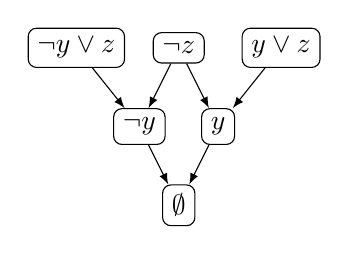
\begin{tikzpicture}[>=latex]
    \node[rectangle, rounded corners = 3pt, draw] (a) at (-1.3, 2)
        {$\neg y \lor z$};
    \node[rectangle, rounded corners = 3pt, draw] (a2) at (1.3, 2)
        {$y \lor z$};
    \node[rectangle, rounded corners = 3pt, draw] (b) at (0, 2)
        {$\neg z$};
    \node[rectangle, rounded corners = 3pt, draw] (c) at (-0.5, 1)
        {$\neg y$};
    \node[rectangle, rounded corners = 3pt, draw] (d) at (0.5, 1)
       {$y$};
    \node[rectangle, rounded corners = 3pt, draw] (e) at (0, 0)
        {$\emptyset$};

    \draw[->] (a) -- (c);
    \draw[->] (a2) -- (d);
    \draw[->] (b) -- (c);
    \draw[->] (b) -- (d);
    \draw[->] (c) -- (e);
    \draw[->] (d) -- (e);
\end{tikzpicture}
    \end{minipage}


    \pause
    \vspace{0.3cm}

    \deftext{Cutting Planes}: proof is a sequence of inequalities over $\mathbb{Z}$
    $(p_1 \ge 0, p_2 \ge 0, p_3 \ge 0, \dots, p_{\ell} \ge 0)$:
    \begin{itemize}
        \item $p_i$ is an encoding of $C \in \varphi$, $x_k \ge 0$ or $-x_k + 1 \ge 0$;
        \item $\frac{p_i ~~~~~ p_j}{p_k}$,  $(p_i \ge 0) \land (p_j \ge 0)$ imply $(p_k \ge 0)$
            \alert{over $\mathbb{Z}^n$};
        \item $p_{\ell} = 1$.
    \end{itemize}
\end{frame}

\begin{frame}{Lower bounds in proof complexity}

    \tikzset{
    >=latex,
    perpinterface/.style = {
        postaction = {
            draw,
            decorate,
            decoration = {
                ticks,
                raise = 0.07cm,
                amplitude = 0.07cm,
                segment length = 1mm
            }
        }
    },
    % пружина
    vert/.style = {
        draw,
        ellipse
    },
    tikzart-fire/.pic = {
        \draw[fill = red!60] (0, 0) .. controls (0.3, 0) and (0.6, 0.1) .. (0.7, 0.3)
            .. controls (0.8, 0.5) and (0.85, 0.6) .. (0.8, 0.9)
            .. controls (0.75, 1.1) and (0.7, 1.2) .. (0.6, 1.4)
            .. controls (0.65, 1.2) and (0.6, 1.05) .. (0.5, 0.9)
            .. controls (0.5, 1.2) and (0.2, 1.3) .. (0.1, 1.6)
            .. controls (0.05, 1.75) and (0.1, 2) .. (0.2, 2.1)
            .. controls (-0.1, 2) and (-0.2, 1.85) .. (-0.3, 1.7)
            .. controls (-0.4, 1.5) and (-0.45, 1.3) .. (-0.4, 1.1)
            .. controls (-0.5, 1.2) and (-0.51, 1.4) .. (-0.5, 1.5)
            .. controls (-0.75, 1.2) and (-0.8, 0.7) .. (-0.7, 0.5)
            .. controls (-0.6, 0.28) and (-0.4, 0) .. (0, 0);
            \fill[white] (0, 0) .. controls (0.3, 0) and (0.52, 0.34) .. (0.37, 0.61)
            .. controls (0.4, 0.54) and (0.32, 0.32) .. (0.25, 0.25)
            .. controls (0.3, 0.35) and (0.25, 0.5) .. (0.2, 0.6)
            .. controls (0.1, 0.8) and (-0.05, 1) .. (0, 1.2)
            .. controls (-0.32, 1) and (-0.3, 0.72) .. (-0.2, 0.47)
            .. controls (-0.3, 0.51) and (-0.31, 0.6) .. (-0.33, 0.7)
            .. controls (-0.4, 0.6) and (-0.4, 0.5) .. (-0.4, 0.4)
            .. controls (-0.35, 0.18) and (-0.2, 0) .. (0, 0);
    }
}


    
\begin{tikzpicture}
    \node[vert] (res) at (1, 0) {$\Res$};
    \node[vert] (ns) at (-3, 0) {$\NS$};
    \node[vert] (cp) at (3, 1) {$\CP$};
    \node[vert] (acf) at (1.2, 1.5) {$\AC_0$-Frege};
    \node[vert] (resl) at (-1, 2.1) {$\ResL$};
    \node[vert] (acfp) at (0.5, 3.5) {$\AC_0[p]$-Frege};
    \node[vert] (fre) at (0.5, 5) {Frege};
    \node[vert] (ips) at (-2, 6) {$\PrSys{IPS}$};
    \node[vert] (pcr) at (-3, 2) {$\PCR[]$};
    \node[vert] (sos) at (-4, 2.5) {$\SOS$};

    \node[vert] (ns2) at (-5.5, 0) {$\NS_{\{\pm 1\}}$};
    \node[vert] (pcr2) at (-6, 2) {$\PCR[]_{\{\pm 1\}}$};
    \node[vert] (sos2) at (-6.8, 3) {$\SOS_{\{\pm 1\}}$};

    \node[vert] (cps) at (-4, 6.5) {$\PrSys{CPS}$};

    \draw[->] (res) -- (cp);
    \draw[->] (cp) to[out = 90, in = -20] (fre);
    \draw[->] (res) -- (resl);
    \draw[->] (res) -- (acf);
    \draw[->] (res) -- (pcr);
    \draw[->] (ns) -- (pcr);
    \draw[->] (resl) -- (acfp);
    \draw[->] (acf) -- (acfp);
    \draw[->] (acfp) -- (fre);
    \draw[->] (fre) -- (ips);
    \draw[->] (ips) -- (cps);

    \draw[->] (pcr) -- (ips);
    \draw[->] (sos) -- (cps);

    \draw[->] (ns2) -- (pcr2);
    \draw[->] (pcr2) -- (ips);
    \draw[->] (sos2) -- (cps);

    \node[inner sep = 0pt] at (-7, 5.5)
    {
\includegraphics[width = .2\textwidth]{pics/dragon.png}};

    \pause
    \draw[ultra thick, blue] (-4, -1) to[out = 110, in = 230] (-4.4, 3) to[out = 50, in = 180] (3.5, 1.8);
    \foreach \point in {(1.5, 3), (-2, 4), (-6, 1)}{
        \pic at \point {tikzart-fire};
    }
    
\end{tikzpicture}
    
\end{frame}

\begin{frame}{Hard formulas for all proof systems}

    \begin{itemize}
        \item If $\varphi$ is unsatisfiable then there is a ``proof'' of unsatisfiability.
            \pause
            \begin{itemize}
                \item \alert{And we can realize it in some proof system...}
            \end{itemize}
            \pause
        \item Distribution on formulas?
            \pause
            \begin{itemize}
                \item Fine. Counting argument do not work in proof complexity.
            \end{itemize}            
    \end{itemize}

    \pause

    \vspace{1cm}
    \begin{itemize}
        \item Random $\Delta$-CNF formulas
        \item Clique formulas
        \item Pseudorandom generator formulas
    \end{itemize}
\end{frame}


\begin{frame}{Random $\Delta$-CNF}

    \begin{minipage}{0.38\linewidth}
        \centering
        \begin{tikzpicture}

    \pgfmathsetseed{1000007}
    \foreach \i in {0, 1, ..., 5}{
        \node[graph-vert] (b\i) at
            (1.5, 0.4 * \i + 0.4) {};
    }

    \foreach \i in {0, 1, 3, 4, ..., 7}{
        \node[graph-vert = {LEIorange!80!black}{0.15cm}] (a\i) at
            (0, 0.4 * \i) {};

        \foreach \j in {0, 1, 2}{
            \pgfmathsetmacro{\temp}{random(0, 5)}
            \draw (a\i) -- (b\temp);
        }
    }

    \node[graph-vert, fill = green!50] (a2) at (0, 0.8) {};
    \foreach \j in {0, 1, 2}{
        \pgfmathsetmacro{\temp}{random(0, 5)}
        \draw[red, thick] (a2) -- (b\temp);
    }

    \node[below = 0.2cm] at (a0) {$m$};
    \node[below = 0.2cm] at (b0) {$n$};
\end{tikzpicture}
    \end{minipage}
    \begin{minipage}{0.58\linewidth}
        \begin{itemize}
            \item $m$ clauses;
            \item $n$ variables;
            \item $\Delta$ neighbours: $\binom{n}{\Delta}$ possibilities;
            \item negations (uniformly at random);
            \item $\mathfrak{D} \coloneqq \frac{m}{n}$ clause density.
        \end{itemize}
    \end{minipage}

    \pause
    \begin{itemize}
        \item $\mathfrak{D} > c_{\Delta} 2^{\Delta} \Rightarrow$ formula is unsat whp;
            \pause
        \item Fiege's conjecture: $\mathfrak{D} = \bigO{1} \Rightarrow$ no poly-time algorithm may
            ``prove'' unsatisfiability of random $\bigO{1}$-CNF.
            \begin{itemize}
                \item Non-approximability of many problems.
            \end{itemize}
    \end{itemize}

\end{frame}




\begin{frame}{Lower bounds in proof complexity}

    
\tikzset{
    vert/.style = {
        draw,
        ellipse
    },
    tikzart-fire/.pic = {
        \draw[fill = red!60] (0, 0) .. controls (0.3, 0) and (0.6, 0.1) .. (0.7, 0.3)
            .. controls (0.8, 0.5) and (0.85, 0.6) .. (0.8, 0.9)
            .. controls (0.75, 1.1) and (0.7, 1.2) .. (0.6, 1.4)
            .. controls (0.65, 1.2) and (0.6, 1.05) .. (0.5, 0.9)
            .. controls (0.5, 1.2) and (0.2, 1.3) .. (0.1, 1.6)
            .. controls (0.05, 1.75) and (0.1, 2) .. (0.2, 2.1)
            .. controls (-0.1, 2) and (-0.2, 1.85) .. (-0.3, 1.7)
            .. controls (-0.4, 1.5) and (-0.45, 1.3) .. (-0.4, 1.1)
            .. controls (-0.5, 1.2) and (-0.51, 1.4) .. (-0.5, 1.5)
            .. controls (-0.75, 1.2) and (-0.8, 0.7) .. (-0.7, 0.5)
            .. controls (-0.6, 0.28) and (-0.4, 0) .. (0, 0);
            \fill[white] (0, 0) .. controls (0.3, 0) and (0.52, 0.34) .. (0.37, 0.61)
            .. controls (0.4, 0.54) and (0.32, 0.32) .. (0.25, 0.25)
            .. controls (0.3, 0.35) and (0.25, 0.5) .. (0.2, 0.6)
            .. controls (0.1, 0.8) and (-0.05, 1) .. (0, 1.2)
            .. controls (-0.32, 1) and (-0.3, 0.72) .. (-0.2, 0.47)
            .. controls (-0.3, 0.51) and (-0.31, 0.6) .. (-0.33, 0.7)
            .. controls (-0.4, 0.6) and (-0.4, 0.5) .. (-0.4, 0.4)
            .. controls (-0.35, 0.18) and (-0.2, 0) .. (0, 0);
    },
    semisim/.style = {
        ->,
        blue,
        dashed,
        decorate,
        decoration = {
            snake,
            amplitude = 0.5,
            segment length = 2
        }
    },        
}


    
\begin{tikzpicture}[xscale = 1.3, xshift = -1]
    \node[vert] (res) at (1, 0) {$\Res$};
    \node[vert] (ns) at (-3, 0) {$\NS$};
    \node[vert] (cp) at (3, 1) {$\CP$};
    \node[vert] (resk) at (1.2, 1.4) {$\Res(k)$};
    \node[vert] (acf) at (1.3, 2.4) {$\AC_0$-Frege};
    \node[vert] (resl) at (-1.3, 2.7) {$\ResL$};
    \node[vert] (acfp) at (0.5, 3.8) {$\AC_0[p]$-Frege};
    \node[vert] (fre) at (0.5, 5) {Frege};
    \node[vert] (ips) at (-2, 6) {$\PrSys{IPS}$};
    \node[vert] (pcr) at (-2.8, 1.9) {$\PCR[]$};
    \node[vert] (sos) at (-4, 2.5) {$\SOS$};
    
    \node[vert] (cps) at (-4, 6.5) {$\PrSys{CPS}$};

    

    \draw[->, semisim] (pcr) -- (sos);
    \draw[->] (res) -- (cp);
    \draw[->] (cp) to[out = 90, in = -20] (fre);
    \draw[->] (res) -- (resl);
    \draw[->] (res) -- (resk);
    \draw[->] (resk) -- (acf);
    \draw[->] (res) to[out = 138, in = -30] (pcr);
    \draw[->] (ns) -- (pcr);
    \draw[->] (resl) -- (acfp);
    \draw[->] (acf) -- (acfp);
    \draw[->] (acfp) -- (fre);
    \draw[->] (fre) -- (ips);
    \draw[->, semisim] (ips) -- (cps);

    \draw[->] (pcr) -- (ips);
    \draw[->] (sos) -- (cps);

    \node at (0, 6.9) {};
    

    \begin{scope}[on background layer]
        \draw[ultra thick, fill = black!10] (-4, -1) to[out = 110, in = 220] (-4.4, 3)
            to[out = 40, in = 200] (-1, 2) to[out = 20, in = 160] (2.3, 3) to[out = -20, in = 90]
            (5, 1) -- (5, -1);
    \end{scope}
    \node[blue] at (-1.5, 0.9) {Lower bounds};


    \pause

    \only<2->{
        \begin{scope}[on background layer]
            \draw[ultra thick, fill = orange!10] (-4, -1) to[out = 110, in = 220] (-4.4, 3)
                to[out = 40, in = 200] (-1, 2) to[out = 20, in = 160] (2.3, 1) to[out = -20, in = 90]
                (5, 1) -- (5, -1);
            \end{scope}
            \node[blue] at (-1.5, 0.5) {Random $\Delta$-CNF};
    }

    \onslide<1->
\end{tikzpicture}
\end{frame}